\chapter{Chapitre 5 : Déploiement et Tests}
\thispagestyle{fancy}
\newpage

La troisième semaine du stage a été consacrée au développement des interfaces utilisateur pour la plateforme d'apprentissage en ligne, ainsi qu'à la mise en place d'un système avancé de traitement des données de contenu. Ces avancées ont permis de construire les fondations interactives de la plateforme et d'optimiser le traitement des ressources pédagogiques.

\section{Intégration et Déploiement du Backend}

La phase de déploiement a impliqué la mise en place de l'infrastructure nécessaire pour héberger et exécuter la plateforme en environnement de production.

\subsection{Configuration du Serveur}

La configuration du serveur a été réalisée en suivant les meilleures pratiques de sécurité et de performance. Les étapes principales ont inclus :

\begin{itemize}
  \item Installation et configuration du système d'exploitation (Linux Ubuntu Server)
  \item Mise en place des règles de pare-feu et de sécurité
  \item Configuration des certificats SSL pour assurer des connexions sécurisées
  \item Installation des dépendances nécessaires au fonctionnement de l'application
  \item Configuration des services de monitoring et de logging
\end{itemize}

\subsection{Déploiement de la Base de Données}

Pour assurer une accessibilité optimale et une scalabilité future, la base de données a été déployée sur MongoDB Atlas, une plateforme de base de données en tant que service (DBaaS). Cette solution cloud offre plusieurs avantages :

\begin{itemize}
  \item Haute disponibilité avec réplication automatique
  \item Surveillance en temps réel des performances
  \item Sauvegardes automatisées
  \item Sécurité renforcée avec authentification et chiffrement
  \item Scalabilité horizontale et verticale selon les besoins
\end{itemize}

\begin{figure}[h!]
  \centering
  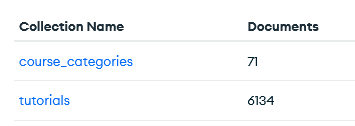
\includegraphics[width=0.9\textwidth,keepaspectratio]{week_3_img/Screenshot 2025-05-19 234047.png}
  \caption{\textbf{Interface MongoDB Atlas} montrant les différentes collections de données.}
  \label{fig:mongodb_collections}
\end{figure}

\subsection{Évolution de l'Architecture}

Après des tests approfondis, une décision stratégique a été prise de migrer d'une architecture MongoDB vers une solution basée sur des fichiers JSON locaux. Cette transition a été motivée par :

\begin{itemize}
  \item La réduction de la complexité architecturale pour la phase actuelle du projet
  \item L'amélioration de l'expérience de développement avec un accès direct aux données
  \item La compatibilité optimale avec le framework Next.js et ses capacités de rendu côté serveur
  \item La simplification du déploiement et de la maintenance pour les premiers stades du projet
\end{itemize}

\section{Intégration et Tests}

\subsection{Tests Unitaires}

Une suite de tests unitaires a été développée pour valider le bon fonctionnement des différents composants de l'application :

\begin{itemize}
  \item Tests des modèles de données
  \item Tests des contrôleurs et services
  \item Tests des utilitaires et fonctions auxiliaires
  \item Tests des composants React avec Jest et React Testing Library
\end{itemize}

\subsection{Tests d'Intégration}

Des tests d'intégration ont été mis en place pour vérifier les interactions entre les différents modules de l'application :

\begin{itemize}
  \item Tests des flux de données entre le frontend et le backend
  \item Tests des interactions avec la base de données
  \item Tests des flux d'authentification et d'autorisation
  \item Tests des processus métier complets
\end{itemize}

\subsection{Tests de Performance}

Des tests de performance ont été réalisés pour s'assurer que l'application répond aux exigences en termes de temps de réponse et de capacité à gérer la charge :

\begin{itemize}
  \item Tests de charge avec simulation d'utilisateurs concurrents
  \item Tests de stress pour identifier les limites de l'application
  \item Analyse des goulots d'étranglement et optimisations nécessaires
  \item Mesure des temps de chargement des pages et des composants
\end{itemize}

\section{Optimisation et Monitoring}

\subsection{Optimisation des Performances}

Plusieurs optimisations ont été apportées pour améliorer les performances de l'application :

\begin{itemize}
  \item Intégration des capacités de rendu côté serveur de Next.js pour améliorer les performances perçues
  \item Mise en place de stratégies de mise en cache pour les données fréquemment accédées
  \item Optimisation des images et des ressources statiques
  \item Implémentation du lazy loading pour les composants non critiques
  \item Minification et bundling des fichiers JavaScript et CSS
\end{itemize}

\subsection{Mise en Place du Monitoring}

Un système de monitoring a été mis en place pour surveiller l'état et les performances de l'application en production :

\begin{itemize}
  \item Intégration de Sentry pour la détection et le suivi des erreurs
  \item Configuration de New Relic pour le monitoring des performances
  \item Mise en place de dashboards de monitoring avec Grafana
  \item Configuration d'alertes en cas de problèmes critiques
  \item Centralisation des logs pour faciliter le débogage
\end{itemize}

\subsection{Documentation}

Une documentation complète a été rédigée pour faciliter la maintenance et l'évolution future de l'application :

\begin{itemize}
  \item Documentation technique de l'architecture
  \item Documentation des API et des endpoints
  \item Guide de déploiement et d'administration
  \item Documentation utilisateur pour les administrateurs de la plateforme
  \item Documentation du processus de développement et des standards de code
\end{itemize}

\section{Conception et Développement de l'Interface Utilisateur}

Après avoir développé la page d'accueil la semaine précédente, l'accent a été mis sur la création des interfaces principales que les utilisateurs utiliseront quotidiennement pour accéder aux contenus et suivre leur progression.

\subsection{Interface d'Accueil des Utilisateurs Connectés}

Une interface d'accueil spécifique pour les utilisateurs connectés a été développée, offrant un accès rapide aux cours en cours, aux recommandations personnalisées et aux dernières activités.

\begin{figure}[h!]
  \centering
  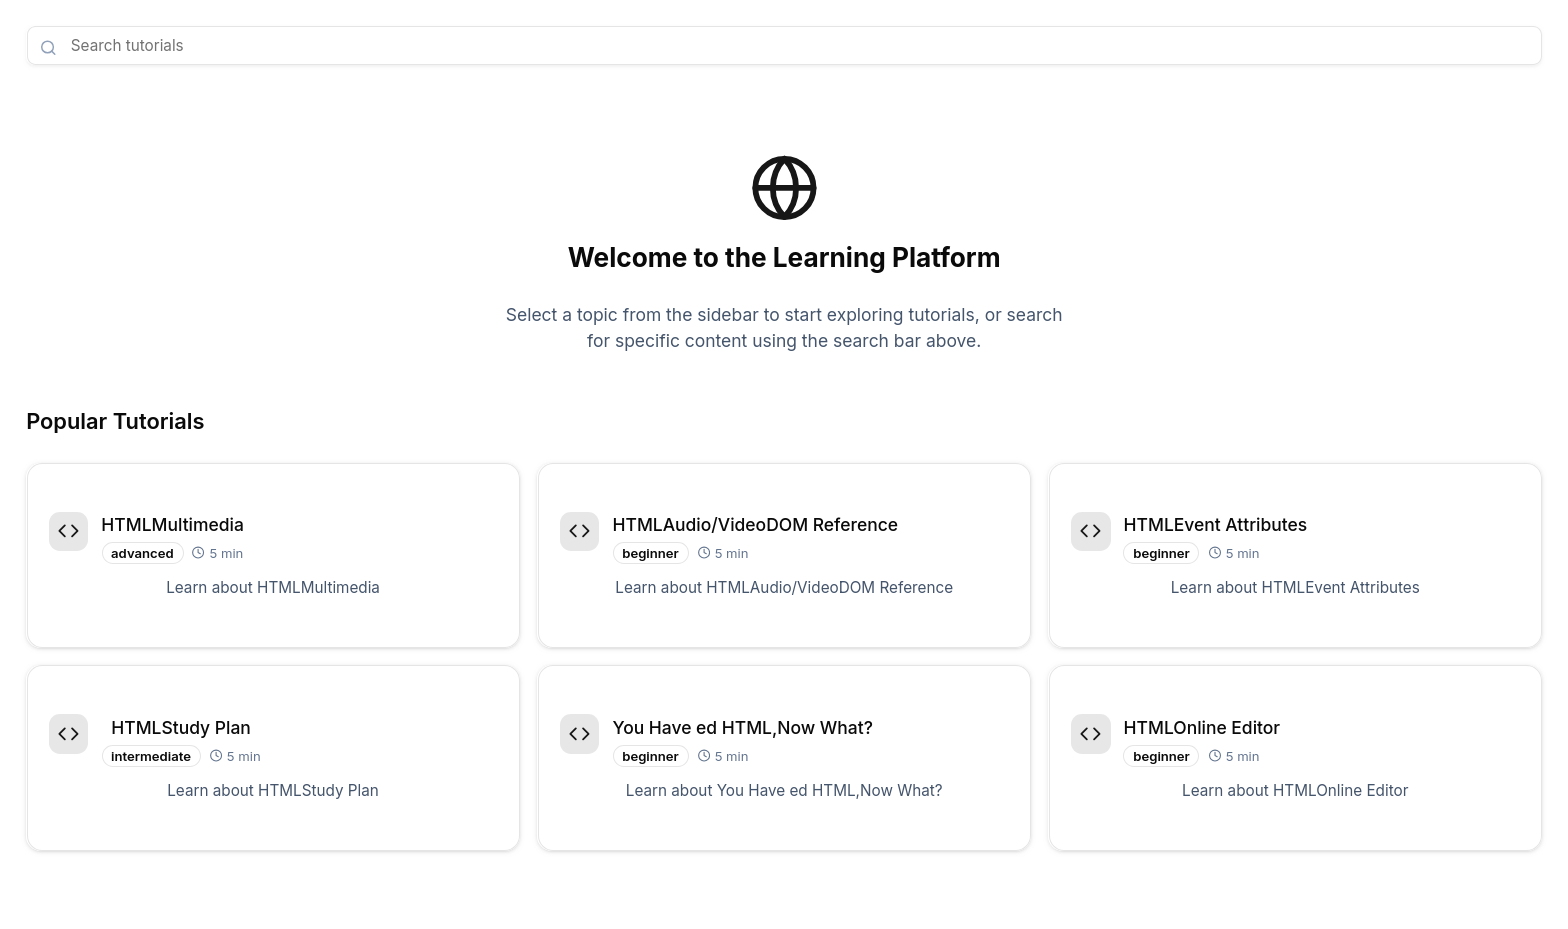
\includegraphics[width=0.9\textwidth,keepaspectratio]{week_3_img/accueil.png}
  \caption{\textbf{Interface d'accueil personnalisée} pour les utilisateurs connectés.}
  \label{fig:user_dashboard}
\end{figure}

\subsection{Barre Latérale de Navigation}

Une barre latérale de navigation intuitive a été implémentée pour faciliter l'accès aux différentes sections de la plateforme.

\begin{figure}[h!]
  \centering
  
\includegraphics[width=0.4\textwidth,keepaspectratio]{week_3_img/sidebare.png}
  \caption{\textbf{Barre latérale de navigation} avec accès aux principales fonctionnalités.}
  \label{fig:sidebar_nav}
\end{figure}

Cette barre latérale comprend :
\begin{itemize}
  \item Accès au tableau de bord personnel
  \item Catalogue de cours et formations
  \item Suivi de progression
  \item Calendrier des sessions de consultation
  \item Paramètres du compte
  \item Centre de notifications
\end{itemize}

\subsection{Interface de Consultation des Cours}

L'interface de consultation des cours a été conçue pour offrir une expérience d'apprentissage immersive et efficace.

\begin{figure}[h!]
  \centering
  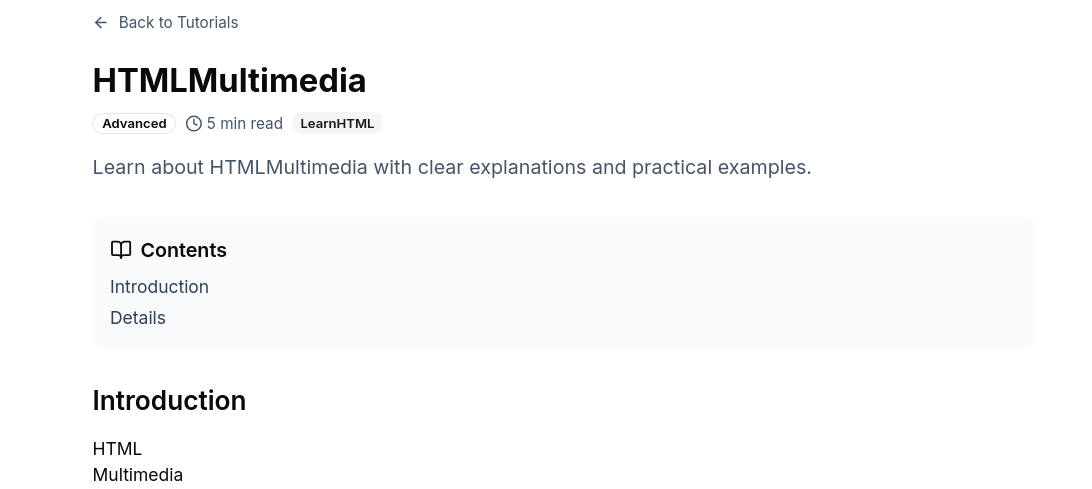
\includegraphics[width=0.9\textwidth,keepaspectratio]{week_3_img/part1.png}
  \caption{\textbf{Interface de consultation des cours} - Partie théorique.}
  \label{fig:course_view_part1}
\end{figure}

\begin{figure}[h!]
  \centering
  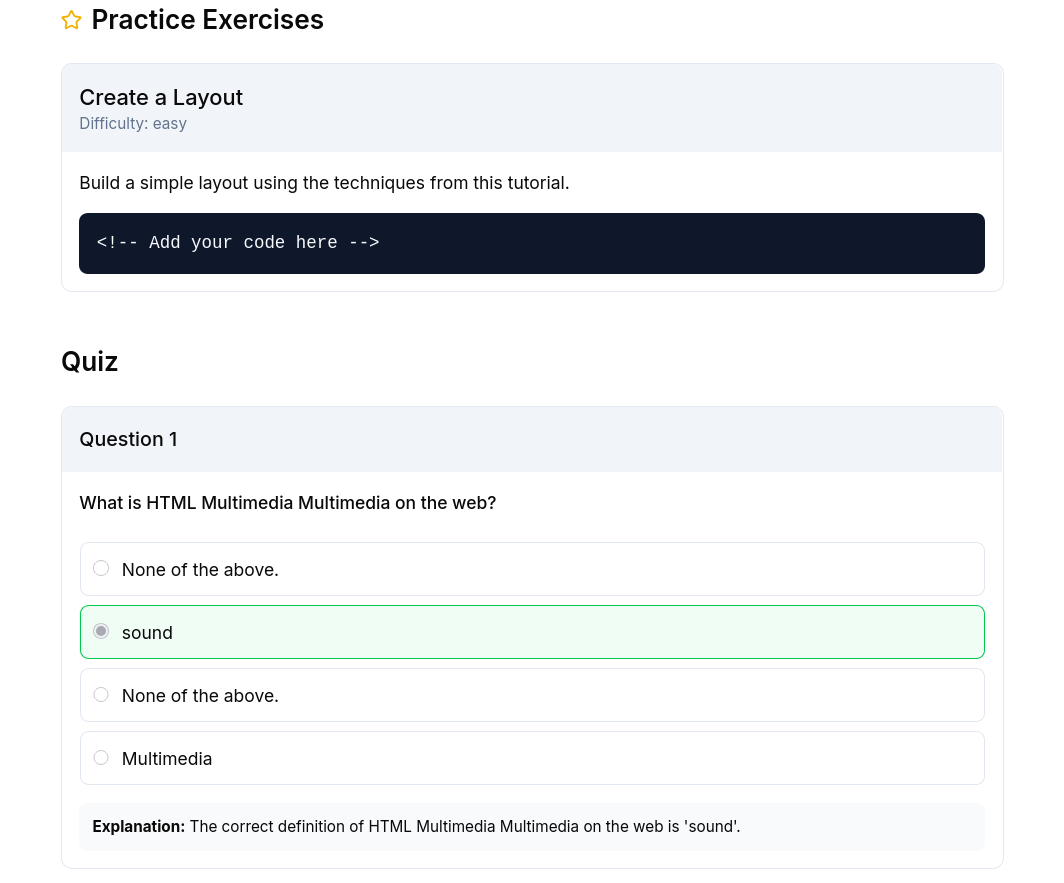
\includegraphics[width=0.9\textwidth,keepaspectratio]{week_3_img/part2.png}
  \caption{\textbf{Interface de consultation des cours} - Partie pratique avec exercices interactifs.}
  \label{fig:course_view_part2}
\end{figure}

Les caractéristiques principales de cette interface incluent :
\begin{itemize}
  \item Affichage clair du contenu théorique avec mise en forme optimisée
  \item Navigation intuitive entre les différentes sections du cours
  \item Exercices interactifs intégrés directement dans l'interface
  \item Suivi de progression en temps réel
  \item Possibilité de prendre des notes contextuelles
  \item Mode sombre/clair pour améliorer le confort de lecture
\end{itemize}

\section{Traitement Avancé des Données de Contenu}

Une partie importante de cette semaine a été consacrée à l'optimisation du traitement des données de contenu éducatif.

\subsection{Défis du Traitement des Données}

Le traitement des données collectées présentait plusieurs défis :
\begin{itemize}
  \item Distinction entre le contenu textuel explicatif et les exemples de code
  \item Structuration cohérente des exemples et exercices
  \item Préservation des formatages spécifiques (tableaux, listes, etc.)
  \item Gestion des caractères spéciaux et encodages
  \item Extraction des métadonnées pertinentes
\end{itemize}

\subsection{Problématique du Scraping et Nettoyage des Données}

L'un des défis majeurs rencontrés a été la séparation du contenu textuel explicatif et des extraits de code dans les sections détaillées des cours. Plusieurs approches ont été explorées :

\begin{itemize}
  \item Tentatives initiales avec des expressions régulières et des algorithmes de traitement de texte, atteignant une précision maximale de 80\%
  \item Expérimentation avec un agent IA basé sur des modèles de langage large (LLM) pour effectuer cette séparation de manière plus intelligente
  \item Découverte finale que la structure HTML particulière de W3Schools nécessitait une approche de scraping spécifique
\end{itemize}

La solution définitive a impliqué une refonte du script de scraping pour mieux cibler les éléments HTML spécifiques, permettant ainsi d'obtenir des données brutes de meilleure qualité dès le départ.

\subsection{Implémentation d'un Pipeline de Traitement LLM}

Pour surmonter ces défis, un pipeline de traitement basé sur des modèles de langage large (LLM) a été conçu et implémenté.

\begin{figure}[h!]
  \centering
  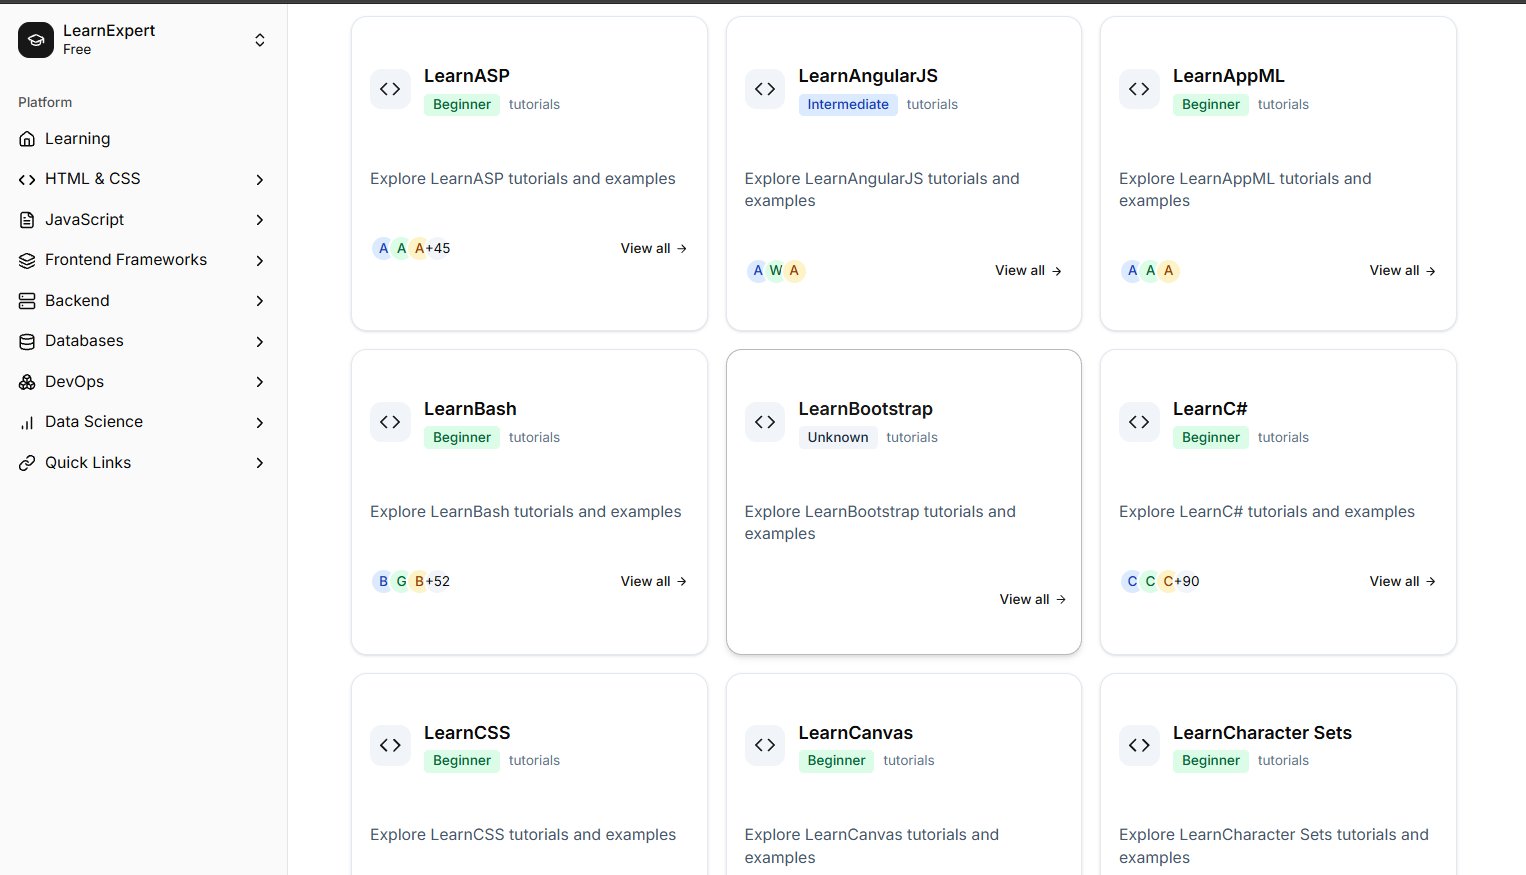
\includegraphics[width=0.9\textwidth,keepaspectratio]{week_3_img/Screenshot 2025-05-20 164411.png}
  \caption{\textbf{Interface d'administration du pipeline LLM} montrant les statistiques de traitement.}
  \label{fig:llm_pipeline}
\end{figure}

\subsection{Stratégie d'Optimisation Multi-LLM}

Le traitement initial utilisant un LLM unique ayant démontré une excellente précision mais des performances limitées en termes de vitesse, une stratégie d'optimisation a été mise en place :

\begin{itemize}
  \item \textbf{Utilisation simultanée de plusieurs fournisseurs LLM :} Parallélisation des requêtes vers différentes API
  \item \textbf{Traitement asynchrone :} Optimisation de la latence perçue en traitant plusieurs segments de données simultanément
  \item \textbf{Segmentation intelligente :} Division des données en unités de traitement optimales pour chaque type de modèle
  \item \textbf{Gestion des requêtes :} Assignation statique de segments spécifiques à des modèles dédiés pour simplifier la gestion de la concurrence
\end{itemize}

Cette approche a permis de réduire significativement le temps de traitement tout en maintenant une qualité optimale, passant d'environ 15 heures à 7-8 heures pour l'ensemble des données.

\section{Intégration Frontend-Backend}

Une attention particulière a été portée à l'intégration efficace entre le frontend et le backend de la plateforme.

\subsection{Développement des Routes d'API}

Des routes d'API RESTful ont été développées pour permettre à l'interface utilisateur d'accéder aux données structurées dans MongoDB :

\begin{itemize}
  \item Routes d'authentification et de gestion des utilisateurs
  \item Routes d'accès au catalogue de cours
  \item Routes de suivi de progression
  \item Routes de gestion des consultations et réservations
  \item Routes d'analytics et de rapports
\end{itemize}

\subsection{Optimisation des Requêtes}

Les requêtes MongoDB ont été optimisées pour garantir des performances optimales :

\begin{itemize}
  \item Création d'index appropriés pour accélérer les recherches fréquentes
  \item Limitation des champs retournés aux données strictement nécessaires
  \item Utilisation de projections pour alléger les transferts de données
  \item Mise en place de pagination pour les listes volumineuses
  \item Implémentation de mécanismes de mise en cache pour les données fréquemment consultées
\end{itemize}

\subsection{Adaptation à l'Architecture JSON}

Suite à la migration vers des fichiers JSON locaux, l'architecture d'accès aux données a été adaptée :

\begin{itemize}
  \item Développement de fonctions de récupération (fetch) optimisées pour les fichiers JSON
  \item Mise en place d'un système de chargement dynamique des données pour les différentes sections de l'interface
  \item Intégration des capacités de rendu côté serveur de Next.js pour améliorer les performances
\end{itemize}

Cette adaptation a permis de maintenir toutes les fonctionnalités prévues tout en simplifiant l'architecture globale du système.

\section{Tests et Validation}

Pour garantir la qualité et la fiabilité des interfaces et systèmes développés, plusieurs types de tests ont été mis en place :

\subsection{Tests d'Interface Utilisateur}

\begin{itemize}
  \item \textbf{Tests de compatibilité :} Vérification du rendu sur différents navigateurs (Chrome, Firefox, Safari, Edge)
  \item \textbf{Tests de responsive design :} Validation de l'adaptation aux différentes tailles d'écran
  \item \textbf{Tests d'accessibilité :} Conformité aux standards WCAG pour garantir l'inclusivité
  \item \textbf{Tests d'utilisabilité :} Évaluation de l'intuitivité et de la fluidité de navigation
\end{itemize}

\subsection{Tests Fonctionnels et d'Intégration}

\begin{itemize}
  \item \textbf{Tests des routes d'API :} Validation des entrées/sorties et gestion des erreurs
  \item \textbf{Tests d'intégration :} Vérification de la communication correcte entre frontend et backend
  \item \textbf{Tests de performance :} Mesure des temps de réponse et optimisation des goulots d'étranglement
  \item \textbf{Tests de charge :} Simulation d'utilisation intensive pour évaluer la robustesse
\end{itemize}

\subsection{Planification Stratégique pour l'Avenir}

En fin de semaine, une réflexion stratégique a été menée concernant l'enrichissement du contenu et la différenciation de la plateforme :

\begin{itemize}
  \item Identification du besoin de diversifier les sources de contenu au-delà de W3Schools
  \item Planification de l'intégration d'éléments interactifs avancés, comme un éditeur de code basé sur les technologies VSCode
  \item Initiation à l'apprentissage des techniques d'optimisation pour les moteurs de recherche (SEO) pour améliorer la visibilité future de la plateforme
\end{itemize}

\section{Conclusion}

Cette troisième semaine a marqué des avancées significatives dans le développement de la plateforme e-learning. La mise en place d'interfaces utilisateur intuitives et ergonomiques, couplée à un système sophistiqué de traitement des données éducatives, a permis de poser les fondations solides pour l'expérience utilisateur finale. L'utilisation innovante de technologies comme MongoDB Atlas et les modèles de langage large (LLM) a apporté des solutions efficaces aux défis techniques rencontrés.

Les interfaces développées durant cette semaine offrent maintenant aux utilisateurs un environnement d'apprentissage fluide et immersif, tandis que l'optimisation du traitement des données garantit une qualité exceptionnelle du contenu éducatif proposé. Les décisions stratégiques prises, notamment la simplification de l'architecture de données et la planification d'éléments différenciateurs, posent les bases d'une plateforme compétitive et évolutive. 